\documentclass{beamer}
\usetheme{Singapore}
\usepackage{changepage}

%\usepackage{pstricks,pst-node,pst-tree}
\usepackage{amssymb,latexsym}
\usepackage{tikz}
\usepackage{graphicx}
\usepackage{fancyvrb}
\usepackage{hyperref}
\usepackage{fancybox}
\usepackage[listings]{tcolorbox}

\definecolor{codegreen}{rgb}{0,0.6,0}
\definecolor{codegray}{rgb}{0.5,0.5,0.5}
\definecolor{codepurple}{rgb}{0.58,0,0.82}
\definecolor{backcolour}{rgb}{0.95,0.95,0.92}

\lstdefinestyle{mystyle}{
    language=Python,
    backgroundcolor=\color{backcolour},   
    commentstyle=\color{codegreen},
    keywordstyle=\color{magenta},
    numberstyle=\tiny\color{codegray},
    stringstyle=\color{codepurple},
    basicstyle=\ttfamily\footnotesize,
    breakatwhitespace=false,         
    breaklines=true,                 
    captionpos=b,                    
    keepspaces=true,                 
    numbers=left,                    
    numbersep=5pt,                  
    showspaces=false,                
    showstringspaces=false,
    showtabs=false,                  
    tabsize=2,
    escapechar=|,
    frame=single
}

\lstset{style=mystyle}


\newcommand{\bi}{\begin{itemize}}
\newcommand{\li}{\item}
\newcommand{\ei}{\end{itemize}}
\newcommand{\Show}[1]{
\begin{center}
\shadowbox{\begin{minipage}{0.8\textwidth}
          #1
          \end{minipage}}
\end{center}
}
\newcommand{\arrow}{\ensuremath{\rightarrow}}

\newcommand{\uparr}{\ensuremath{\uparrow}}


\newcommand{\fig}[2]{\centerline{\includegraphics[width=#1\textwidth]{#2}}}

\newcommand{\bfr}[1]{\begin{frame}[fragile]\frametitle{{ #1 }}}
\newcommand{\efr}{\end{frame}}

\newcommand{\cola}{\begin{columns}\begin{column}{0.5\textwidth}}
\newcommand{\colb}{\end{column}\begin{column}{0.5\textwidth}}
\newcommand{\colc}{\end{column}\end{columns}}


\title{Think Python 2e, Chapter 10 Notes}
\author{Lists}

\begin{document}

\begin{frame}
\maketitle
\end{frame}

\bfr{Lists}
\begin{lstlisting}
>>> cheeses = ['Cheddar', 'Edam', 'Gouda']
>>> numbers = [42, 123]
>>> empty = []
>>> print(cheeses, numbers, empty)
['Cheddar', 'Edam', 'Gouda'] [42, 123] []
>>> mixed_list = ['spam', 2.0, 5, [10, 20]]
\end{lstlisting}
\bi
\li A sequence of values, called {\bf elements} or {\bf items}
\li Values of elements in a list can be anything.
\li A list in a list is called {\bf nested}
\li The empty list is just \lstinline{[]}
\ei
\end{frame}

\bfr{Lists are mutable}
\cola
\begin{lstlisting}
>>> cheeses = ['Cheddar', 'Edam', 'Gouda']
>>> numbers = [42, 123]
>>> empty = []
>>> numbers[1] = 5
\end{lstlisting}
\colb
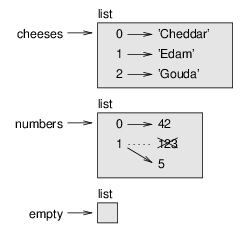
\includegraphics{statediagram10-1}
\colc
\end{frame}

\bfr{Indexing the same in lists and strings}

\bi
\li Any integer expression can be used as an index.
\li If you try to read or write an element that does not exist, you get an IndexError.
\li If an index has a negative value, it counts backward from the end of the list.
\li Slicing works the same.
\ei

\begin{lstlisting}
>>> foo = ['hello', 'there', 'how', 'are', 'you?']
>>> foo[2:4]
['how', 'are']
\end{lstlisting}

\end{frame}
\bfr{The in operator also works on lists.}

\begin{lstlisting}
>>> cheeses = ['Cheddar', 'Edam', 'Gouda']
>>> 'Edam' in cheeses
True
>>> 'Brie' in cheeses
False
\end{lstlisting}

\end{frame}
\bfr{The math operators also work on lists.}

\begin{lstlisting}
>>> [1,2] + [3,4]
[1, 2, 3, 4]
>>> [1, 2, 3] * 3
[1, 2, 3, 1, 2, 3, 1, 2, 3]
\end{lstlisting}

\end{frame}

\bfr{List traversal}
\begin{lstlisting}
for cheese in cheeses:
    print(cheese)
\end{lstlisting}
\begin{lstlisting}
for i in range(len(numbers)):
    numbers[i] = numbers[i] * 2
\end{lstlisting}
\end{frame}


\bfr{Traversal only happens at top level}
\begin{lstlisting}
>>> x = [1,2,3]
>>> y = ['hello','bye']
>>> a = [99, x, y, 100]
>>> a
[99, [1, 2, 3], ['hello', 'bye'], 100]
>>> for item in a:
             print(item)
99
[1, 2, 3]
['hello', 'bye']
100
\end{lstlisting}

\end{frame}

\bfr{List methods}
\begin{lstlisting}
>>> t = ['a', 'b', 'c']
>>> t.append('d')
>>> t
['a', 'b', 'c', 'd']
\end{lstlisting}
\begin{lstlisting}
>>> t1 = ['a', 'b', 'c']
>>> t2 = ['d', 'e']
>>> t1.extend(t2)
>>> t1
['a', 'b', 'c', 'd', 'e']
\end{lstlisting}
{\tt t2} is unmodified
\end{frame}
\bfr{List methods}

\begin{lstlisting}>>> t = ['d', 'c', 'e', 'b', 'a']
>>> t.sort()
>>> t
['a', 'b', 'c', 'd', 'e']
\end{lstlisting}
\pause
\bigskip

\centerline{
\shadowbox{
NO! $\Rightarrow$ \fbox{\lstinline{t = t.sort()}} $\Leftarrow$ BAD!}}

\end{frame}

\bfr{Reduce}

Converting a list of numbers to a single number.

\begin{lstlisting}
def add_all(t):
    total = 0
    for x in t:
        total += x
    return total
\end{lstlisting}

\bigskip

The augmented assignment statement:
\begin{lstlisting}
total += x
\end{lstlisting}
equivalent to
\begin{lstlisting}
total = total + x
\end{lstlisting}

\pause
This is so common python provides a builtin function:
\begin{lstlisting}
>>> t = [1, 2, 3]
>>> sum(t)
6
\end{lstlisting}



\end{frame}
\bfr{Reduce}

Converting a list of strings to a single string.

\begin{lstlisting}
def cat_all(t):
    total = ''
    for x in t:
        total += x
    return total
\end{lstlisting}
\begin{lstlisting}
>>> cat_all(['hello','there','how','are','you'])
'hellotherehowareyou'
\end{lstlisting}


\bigskip
\pause

This is so common python provides a builtin:
\begin{lstlisting}
>>> x = ['hello', 'there', 'how', 'are', 'you']
>>> ''.join(x)\
'hello/there/how/are/you'
>>> '   '.join(x)
'hello   there   how   are   you'\
\end{lstlisting}


\end{frame}

\bfr{Map}

Traverse one list while building another.
\begin{lstlisting}
def capitalize_all(t):
    res = []
    for s in t:
        res.append(s.capitalize())
    return res
\end{lstlisting}

\begin{lstlisting}
>>> capitalize_all(['hello','there'])
['Hello', 'There']
\end{lstlisting}

\end{frame}

\bfr{Filter}
Select only some elements of a list.
\begin{lstlisting}
def only_upper(t):
    res = []
    for s in t:
        if s.isupper():
            res.append(s)
    return res
\end{lstlisting}
\begin{lstlisting}
>>> only_upper(['hello', 'BOB', 'hello', 'HELLO']
['BOB', 'HELLO']
\end{lstlisting}


\end{frame}

\bfr{Map, Filter, Reduce}
\bi
\li Paradigms of functional programming
\li Structure complex programs
\li Used in large-scale parallel programming
\ei

\end{frame}

\bfr{Deleting elements: {\tt pop}}

Deletes and returns one element.

\begin{lstlisting}
>>> t = ['a', 'b', 'c']
>>> x = t.pop(1)
>>> t
['a', 'c']
>>> x
'b'
\end{lstlisting}
Without optional parameter, deletes the last one
\begin{lstlisting}
>>> t = [1,2,3]
>>> t.pop()
3
>>> t
[1, 2]
\end{lstlisting}

\end{frame}
\bfr{Deleting elements: {\tt del}}

If you don't need the removed value, use {\tt del}

\begin{lstlisting}
>>> t = ['a', 'b', 'c']
>>> del t[1]
>>> t
['a', 'c']
\end{lstlisting}

Can delete slices
\begin{lstlisting}
>>> t = ['a', 'b', 'c', 'd', 'e', 'f']
>>> del t[1:5]
>>> t
['a', 'f']
\end{lstlisting}

\end{frame}

\bfr{Deleting elements: {\tt remove}}

If you know the element but not the index, use {\tt remove}

\begin{lstlisting}
>>> t = ['a', 'b', 'c']
>>> t.remove('b')
>>> t
['a', 'c']
\end{lstlisting}

The return value is {\tt None}

\end{frame}

\bfr{Lists and Strings}

\begin{lstlisting}
>>> s = 'spam'
>>> t = list(s)
>>> t
['s', 'p', 'a', 'm']
\end{lstlisting}

\begin{lstlisting}
>>> s = 'pining for the fjords'
>>> t = s.split()
>>> t
['pining', 'for', 'the', 'fjords']
\end{lstlisting}

\begin{lstlisting}
>>> s = 'spam-spam-spam'
>>> delimiter = '-'
>>> t = s.split(delimiter)
>>> t
['spam', 'spam', 'spam']
\end{lstlisting}

\end{frame}
\bfr{Lists and Strings}

\begin{lstlisting}
>>> t = ['pining', 'for', 'the', 'fjords']
>>> delimiter = ' '
>>> s = delimiter.join(t)
>>> s
'pining for the fjords'
\end{lstlisting}

\end{frame}

\bfr{Objects and values}

\begin{lstlisting}
>>> a = 'banana'
>>> b = 'banana'
>>> a == b
True
\end{lstlisting}

Which is the case?

{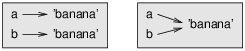
\includegraphics{statediagram10-2}}

\pause
Check with {\tt is} operator:
\begin{lstlisting}
>>> a is b
True
\end{lstlisting}

Python only creates one string.


\end{frame}

\bfr{Lists are different}
\begin{lstlisting}
>>> a = [1, 2, 3]
>>> b = [1, 2, 3]
>>> a == b
True
>>> a is b
False
\end{lstlisting}

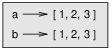
\includegraphics{statediagram10-3}

\bi
\li
They are {\bf equivalent} but not {\bf identical}.
\li
We say that an {\bf object} has a {\bf value}.
\ei
\end{frame}

\bfr{Aliasing}

\cola
\begin{lstlisting}
>>> a = [1, 2, 3]
>>> b = a
>>> b is a
True
\end{lstlisting}
\colb
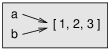
\includegraphics{statediagram10-4}
\colc

\bi
\li Association of a variable with an object is called a {\bf reference}
\li If there is more than one reference, an object is {\bf aliased}.
\li Changes to one change all aliases:
\ei
\begin{lstlisting}
>>> b[0] = 42
>>> a
[42, 2, 3]
\end{lstlisting}
\bi
\li Aliasing is dangerous
\ei


\end{frame}

\bfr{List arguments are aliased}


\begin{lstlisting}
def delete_head(t):
    del t[0]
\end{lstlisting}
\begin{lstlisting}
>>> letters = ['a', 'b', 'c']
>>> delete_head(letters)
>>> letters
['b', 'c']\end{lstlisting}

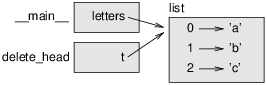
\includegraphics{statediagram10-5}

\end{frame}

\bfr{Destructive operations}


\begin{lstlisting}
>>> t1 = [1, 2]
>>> t2 = t1.append(3)
>>> t1
[1, 2, 3]
>>> t2
None
>>> t3 = t1 + [4]
>>> t1
[1, 2, 3]
>>> t3
[1, 2, 3, 4]
\end{lstlisting}


\bi
\li The {\tt append} operation destroys the original list {\tt t1}
\li The {\tt + } operation does not
\ei


\end{frame}

\bfr{Functions that (don't) modify lists}

\begin{lstlisting}
def bad_delete_head(t):
    t = t[1:]              # WRONG!
\end{lstlisting}
\begin{lstlisting}
>>> t4 = [1, 2, 3]
>>> bad_delete_head(t4)
>>> t4
[1, 2, 3]
\end{lstlisting}



\end{frame}

\bfr{Usually better to create new lists}

\begin{lstlisting}
def tail(t):
    return t[1:]
\end{lstlisting}
\begin{lstlisting}
>>> letters = ['a', 'b', 'c']
>>> rest = tail(letters)
>>> rest
['b', 'c']
\end{lstlisting}


\end{frame}

\bfr{Most list methods return {\tt None}}

\begin{lstlisting}
word = word.strip()         # RIGHT!
t = t.sort()                # WRONG!
\end{lstlisting}

\pause
Sometimes desctructive and nondestrucitve versions exist
\begin{lstlisting}
>>> t = [3,5,2,1,4]
>>> s = sorted(t)
>>> t
 [3,5,2,1,4]
>>> s
[1,2,3,4,5]
\end{lstlisting}




\end{frame}

\bfr{Pick an idiom and stick with it}
\bi
\li
There are too many confusing ways to do things sometimes.
\li
Removing elements from lists:
\bi
\li {\tt pop}
\li {\tt remove}
\li {\tt del}
\li slice assignment
\ei
\pause
\li {\bf Pick one!}
\ei


\end{frame}

\bfr{Make copies to avoid aliasing}
\begin{lstlisting}
>>> t = [3, 1, 2]
>>> t2 = t[:]
>>> t2.sort()
>>> t
[3, 1, 2]
>>> t2
[1, 2, 3]
\end{lstlisting}

\end{frame}

\bfr{Vocabulary}
\begin{description}
\li[list:]
A sequence of values.
\li[element:]
One of the values in a list (or other sequence), also called items.
\li[nested list:]
A list that is an element of another list.
\li[accumulator:]
A variable used in a loop to add up or accumulate a result.
\li[augmented assignment:]
A statement that updates the value of a variable using an operator like +=.
\end{description}
\end{frame}
\bfr{Vocabulary}
\begin{description}
\li[reduce:]
A processing pattern that traverses a sequence and accumulates the elements into a single result.
\li[map:]
A processing pattern that traverses a sequence and performs an operation on each element.
\li[filter:]
A processing pattern that traverses a list and selects the elements that satisfy some criterion.

\end{description}
\end{frame}
\bfr{Vocabulary}
\begin{description}
\li[object:]
Something a variable can refer to. An object has a type and a value.
\li[equivalent:]
Having the same value.
\li[identical:]
Being the same object (which implies equivalence).
\li[reference:]
The association between a variable and its value.
\li[aliasing:]
A circumstance where two or more variables refer to the same object.
\li[delimiter:]
A character or string used to indicate where a string should be split.
\end{description}
\end{frame}

\end{document}
